\section{Proposed Algorithm}
\label{sec:algorithm}


Our proposed algorithm consists of two main parts:
a) a FCN-style network providing a coarse segmentation of synaptic cleft;
b) a contour growing technique that uses the coarse segmentation as a start point to extract the whole contours of the synaptic cleft region.
The pipeline of our framework is illustrated in Fig.~\ref{fig:cg}.

\subsection{Pre-segmentation}

To accurately localize the location of target regions, an FCN-style network is first implemented to provide a coarse segmentation for synaptic cleft.
The architecture of the networks are based on DeepLab (ResNet-101)~\cite{Chen2016a}, which uses the dilated convolution for lager receptive fields. 
%
We also explore the effects of different networks to our framework in Sec.~\ref{sec:experiments} to demonstrate the robustness of our model.
%
For the synaptic cleft segmentation, we modify the classifier of DeepLab to a binary classifier and use a weighted loss for mitigating the unbalanced label problem in our task.
For the problem of limited data caused by the expensive acquisition, the transfer learning strategy is used by fine-tuning the weights of lower layers on the off-the-shelf model from DeepLab, which have been well trained on natural images.

\xj{What happens if there are multiple cleft regions?}



\subsection{Contour growing}

Based on the binary mask from pre-segmentation, we first generate an \change{initial centric curve} from the mask, which will be subsequently evolved to the target contours.
%
In order to make sure that the initial centric curve is inside the cleft region, it will be generated as short as possible, such as the green dotted line in Fig.~\ref{fig:cg}.
\xj{How do you determine the length? a fixed length? or a fixed ratio?}
%
The initial centric curve is evolved to respectively attach to the presynaptic and postsynaptical membranes, which are exactly the contours of synaptic cleft.
%
Then the contours at both sides are extended synchronously to extract the whole synaptic cleft region.
 



\subsubsection{Curve evolving}
\label{sec:curve_evolving}


Similar to the traditional snake model~\cite{Kass1988}, the initial centric curve is expressed by a parameterized model $\mathbf{v}(s)=\big(x(s),y(s)\big)$, where $s\in[0,1]$ is the arc-length along the curve.
Our goal is to minimize the following energy function:
\begin{eqnarray}\label{Eq:Etotal}
E_{total} =&\int_{0}^{1} E_{int}\big( \vb{v}(s) \big)+ E_{ext}\big( \mathbf{v}(s)\big) ds \\
E_{int} = & \alpha\mathbf{v}^{'}(s)+\beta\mathbf{v}^{''}(s) \\\nonumber
E_{ext} =& I\big( \mathbf{v}(s)\big) + \kappa G\big(\mathbf{v}(s)\big),\nonumber
\end{eqnarray}
where $\mathbf{v}^{'}(s)$ and $\mathbf{v}^{''}(s)$ are the first-order and second-order derivatives of $\mathbf{v}(s)$.
$I$ is the Gaussian smoothed image.
$G$ is the gradient magnitude map.
\xj{The first term tends to smooth curve?... The second term tends to dark and smooth regions?}
According to \cite{Kass1988}, Eq.~\ref{Eq:Etotal} can be minimized by iteratively updating the following equation:
\begin{eqnarray}\label{Eq:GVF}
\mathbf{v}_{t+1}(s) = (\vb{A}+\gamma \vb{I})^{-1}(\gamma \mathbf{v}_t(s)+\mathbf{f}\{\mathbf{v}_t(s)\}),
\end{eqnarray}
where $\vb{A}$ is a matrix encoding the internal tension, $\gamma$ controls the evolving rate and $\mathbf{f}=[f_{x},f_{y}]$ are the gradient maps calculated from $E_{ext}$ using Gradient Vector Flow (GVF) algorithm \cite{Xu1998}.

The updating strategy of Eq.~\ref{Eq:GVF} is very sensitive to the noise, which easily traps some control points.
And the capture range of tension $\mathbf{f}$ is usually limited \cite{Cohen1991}, making its performance depend heavily on the initial curve.
Our experiments illustrate the deficiencies of GVF in detail and show some representative cases in Fig.~\ref{fig:gvf}.
Thus in this section, we propose a new updating strategy by:
\begin{eqnarray}\label{Eq:update}
\mathbf{v}_{t+1}(s) = (A+\gamma I)^{-1}(\gamma \mathbf{v}_t(s)+E_{ext}\{\mathbf{v}(s)\}\mathbf{n}\{\mathbf{v}_t(s)\})
\end{eqnarray}
$\mathbf{n}\{\mathbf{v}(s)\}$ are the normal vectors of $\mathbf{v}(s)$ with consistent orientations.

In Eq.~\ref{Eq:update}, the direction of external tension are fixed as the normal direction of $\mathbf{v}_(s)$, whose magnitudes are controlled by $E_{ext}\{\mathbf{v}(s)\}$ instead of a constant value in Ballons model \cite{Cohen1991}.
The advantages of Eq.~\ref{Eq:update} are follows:
a) the capture range of external tension are much larger, due to fixed tension $\mathbf{n}\{\mathbf{v}(s)\}$;
b) it is easier to reach the global optimum than GVF, because $E_{ext}$ will soon vanish in the contour region;
c) In the noise region, once the internal tension pulls a trapped $\mathbf{v}(s)$ out, our external tension will soon push it away.
The above situations are shown in Fig.~\ref{fig:gvf}.



\begin{figure}[t]
	\begin{center}
		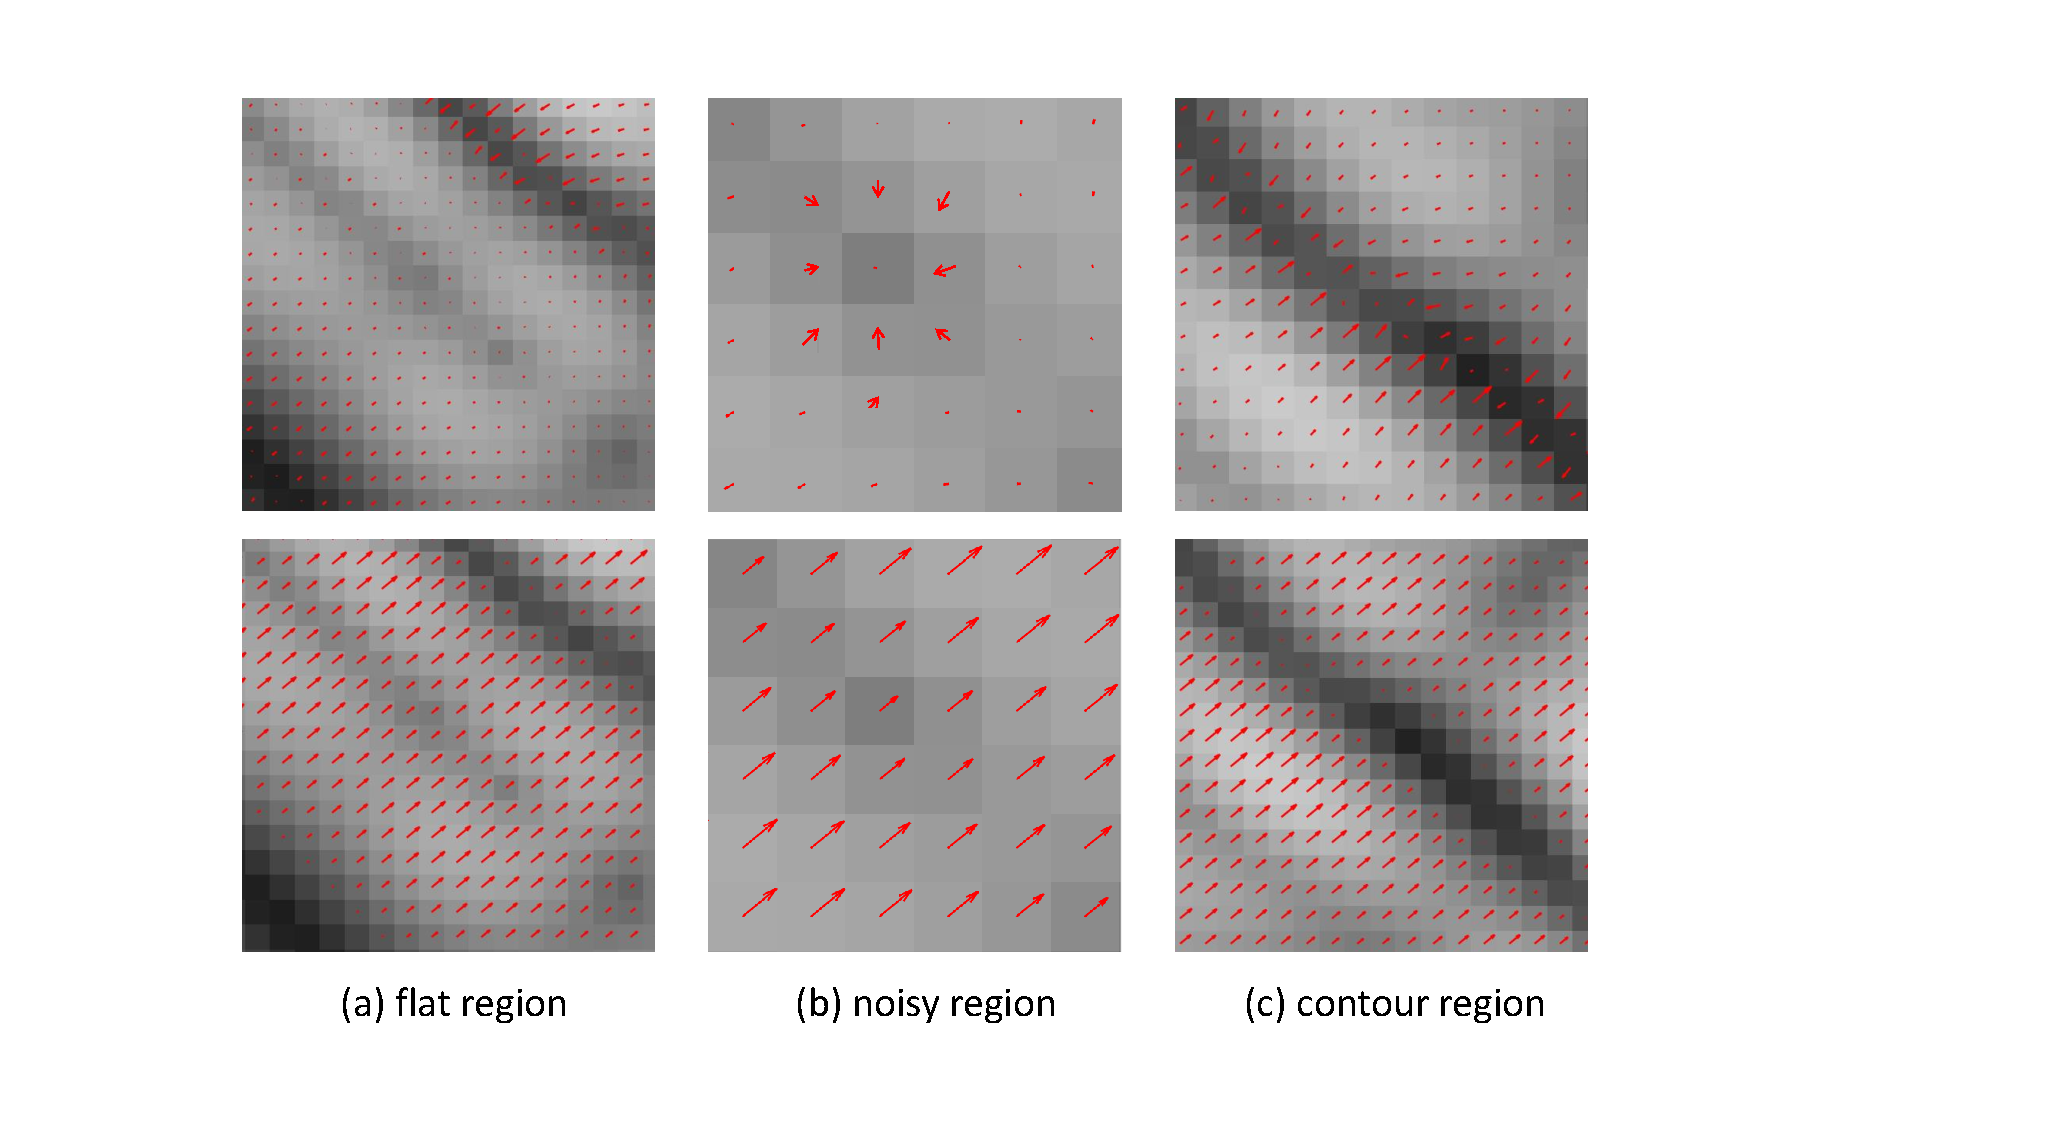
\includegraphics[width=3.4in]{figs/FigGVF.pdf}
	\end{center}
	%
	\caption{Several cases of tension field obtained by GVF (top row) and our normal force (bottom row). The red arrow indicates the force vector of external tension.}
	\label{fig:gvf}
\end{figure}



By setting opposite normal vectors ($\mathbf{n}_{+}$ and $\mathbf{n}_{-}$ in Figure~\ref{fig:cg}), $\mathbf{v}(s)$ will be evolved along opposite direction and well attach to both presynaptic and postsynaptical membranes.
The final evolved curves are respectively denoted as $\mathbf{c}_1(s)$ and $\mathbf{c}_2(s)$.

\begin{figure}[t]
\begin{minipage}[b]{1.0\linewidth}
  \centering
 \centerline{\epsfig{figure=Figs/FigG.pdf,width=8.5cm}}
\end{minipage}
\caption{An example of contour growing formulated by Eq.~\ref{Eq:sg}.
        The yellow solid arrow indicates the growing direction of previous stages.
        The dotted arrows visualize the candidates of next growing direction, and the direction with the darkest color is our preferred.
        After finding the optimal length, the longest arrow is chosen as a new piece of growing contour.}
\label{fig:g}
\end{figure}

\subsubsection{Synchronous growing}
With two pieces of contour $\mathbf{c}_1(s)$ and $\mathbf{c}_2(s)$, we then grow them to localize the whole presynaptic and postsynaptic membranes.
The challenge of this part is that they should be grown correctly and synchronously to compute the exact distance between two membranes for termination judging.

First, we formulate the process of growing $\mathbf{c}_1(s)$ as finding a piece of straight line $\mathbf{l}(s)$ by:
\begin{eqnarray}\label{Eq:sg}
&\arg\min_{\mathbf{l}(s)} E_{int}\{\mathbf{l}(s)+c_1(1))\}+\rho(\overrightarrow{c_1}(1)*\overrightarrow{l}(0))\\
&st.~\tau_1\leq (\overrightarrow{c_1}(0)*\overrightarrow{l}(0))\leq \tau_2\nonumber
\end{eqnarray}
where $*$ defines the inner product of two vectors.
$c_1(1)$ is the end point of curve $\mathbf{c}_1$ and $\overrightarrow{c_1}(1)$ is the tangent vector of point $c_1(1)$.
Especially, $\mathbf{l}(s)$ can be expressed by a direction vector $\overrightarrow{l}(0))$ and a length variable $l$.
The firs term of Eq.~\ref{Eq:sg} expects the $\mathbf{l}(s)$ to grow along the membranes with low $E_{ext}$, while the second term hope the grow direction to follow the previous direction.
$\rho$ is a tradeoff parameter, and $\tau_1,\tau_2$ add a hard restraint on the growing direction to be not changed too much.

Optimal solution of Eq.~\ref{Eq:sg} can be obtained by using the EM algorithm.
Explicitly, we first fixed $l$ to find an optimal $\overrightarrow{l}(0))$, and then fix $\overrightarrow{l}(0))$ to find a better $l$.
Experiments show that two times of iteration is enough for most cases to give a satisfying piece of new growing membrane as shown in Fig.~\ref{fig:g}.

Next to synchronously grow $\mathbf{c}_1(s)$ and $\mathbf{c}_2(s)$, we split the growing process into several periods and decide which curve grows in each period.
Especially, we set two variables $g_1^{t+1}$ and $g_2^{t+1}$  ($1$ for growing and $0$ for waiting) to determine the growing state of $\mathbf{c}_1^{t}(s)$ and $\mathbf{c}_2^{t}(s)$ at stage $t+1$ by:
\begin{eqnarray}\label{Eq:gf}
g_1^{t+1},g_2^{t+1} = \left\{\begin{array}{cc}
0,1&if \overrightarrow{c}^t_1(1)*(c_2^t(1)-c_1^t(1))\geq 0 \\
1,0&if \overrightarrow{c}^t_1(1)*(c_2^t(1)-c_1^t(0))\leq 0\\
1,1& else\\
\end{array}\right.
\end{eqnarray}
where $c_1^t(0)$, $c_1^t(1)$ and $c_2^t(1)$ are three endpoints of two growing membranes as shown in Figure~\ref{fig:sg}.
Different situations of Eq.~\ref{Eq:gf} are shown in Figure~\ref{fig:sg}.
And the distance between two membranes can be then calculated by:
\begin{eqnarray}\label{Eq:d}
d^{t+1} = \frac{||c_1^{t+1}(1)-c_2^{t+1}(1)||+ ||c_1^{t+1}(0)-c_2^{t+1}(0)||}{2}
\end{eqnarray}
Once $d^{t+1}$ is beyond the range of reasonable cleft width, the growing will be terminated.
\begin{figure}[t]
\begin{minipage}[b]{1.0\linewidth}
  \centering
 \centerline{\epsfig{figure=Figs/FigSG.pdf,width=8.5cm}}
\end{minipage}
\caption{Diagram of different situations illustrated in Eq.~\ref{Eq:gf}.
        The green lines are the new growing contour, while the red lines are the previous contours}
\label{fig:sg}
\end{figure}
